% Submissions for peer-review must enable line-numbering 
%% using the lineno option in the \documentclass command.
%%
%% Preprints and camera-ready submissions do not need 
%% line numbers, and should have this option removed.
%%
%% Please note that the line numbering option requires
%% version 1.1 or newer of the wlpeerj.cls file, and
%% the corresponding author info requires v1.2

\documentclass[fleqn,10pt,lineno]{wlpeerj} % for journal submissions
% \documentclass[fleqn,10pt]{wlpeerj} % for preprint submissions

%\usepackage{hyperref}
\usepackage{setspace}
% \usepackage{gensymb}
% \usepackage{xcolor} % added by NJG for edits

\title{Draft \textit{Aphaenogaster} genomes expand our view of ant
  genome size variation across climate gradients}

\author[1]{Matthew K. Lau}
\author[1]{Aaron M. Ellison}
\author[2,3]{Andrew D. Nguyen}
\author[4,5]{Clint Penick}
\author[6]{Bernice DeMarco}
\author[2]{Nicholas J. Gotelli}
\author[7]{Nathan J. Sanders}
\author[4]{Robert R. Dunn}
\author[2]{Sara Helms Cahan}

\affil[1]{Harvard Forest, Harvard University, Petersham, MA, USA}
\affil[2]{Department of Biology, University of Vermont, Burlington,
  VT, USA}
\affil[3]{Department of Entomology and Nematology, University of
  Florida, Gainesville, FL, USA}
\affil[4]{Department of Applied Ecology, North Carolina State
  University, Raleigh, NC, USA}
\affil[5]{The Biomimicry Center, Arizona State University, Tempe, AZ, USA}
\affil[6]{Smithsonian Institution, Washington, DC, USA}
\affil[7]{Environmental Program, Rubenstein School of Environment and
  Natural Resources, University of Vermont, Burlington, VT, USA}

\corrauthor[]{Matthew K. Lau}{matthewklau@fas.harvard.edu}

%% \keywords{genomics, biogeography, climate change, ants, Formcicidae}
\begin{abstract}

Given the abundance, broad distribution, and diversity of roles that
ants play in many ecosystems, they are an ideal group to serve as
ecosystem indicators of climatic change. At present, only a few
whole-genome sequences of ants are available (19 of $>$ 16,000
species), mostly from tropical and sub-tropical species.  To address
this limited sampling, we sequenced genomes of temperate-latitude
species from the genus \textit{Aphaenogaster}, a genus with important
seed dispersers. In total, we sampled seven colonies of six species:
\textit{A. ashmeadi}, \textit{A. floridana}, \textit{A. fulva},
\textit{A. miamiana}, \textit{A. picea}, and \textit{A. rudis}. The
geographic ranges of these species collectively span eastern North
America from southern Florida to southern Canada, which encompasses a
latitudinal gradient in which many climatic variables are changing
rapidly. For the six genomes, we assembled an average of 271,039
contigs into 47,337 scaffolds. The mean genome size was 370.5 Mb,
ranging from 310.3 to 429.7, which is comparable to that of other
sequenced ant genomes (212.8 to 396.0 Mb) and flow cytometry estimates
(210.7 to 690.4 Mb). In an analysis of currently sequenced ant genomes
and the new \textit{Aphaenogaster} sequences, we found that after
controlling for both spatial autocorrelation and phylogenetics ant
genome size was marginally correlated with sample site climate
similarity. Of all examined climate variables, minimum temperature
showed the strongest correlation with genome size, with ants from
locations with colder minimum temperatures having larger
genomes. These results suggest that temperature extremes could be a
selective force acting on ant genomes and point to the need for more
extensive sequencing of ant genomes.

\end{abstract}

\begin{document}

\flushbottom
\maketitle
\thispagestyle{empty}

%% \subsection*{About PeerJ}

%% PeerJ is an award-winning open access publisher covering the
%% biological and medical sciences.  PeerJ provides authors with three
%% publication venues: \textit{PeerJ} and \textit{PeerJ Computer Science}
%% (peer-reviewed academic journals) and \textit{PeerJ PrePrints} (a
%% 'pre-print server'). See https://peerj.com/about/publications/ for
%% more information.

%% The PeerJ model allows an author to publish articles in their
%% peer-reviewed journal via the purchase of a lifetime Publication
%% Plan. Prices start from just \$99 (a one-off payment) which entitles
%% an author to the lifetime ability to publish 1 article per year for
%% free. Publication in PeerJ PrePrints is entirely free.

%% If you have a question, please use the help menu in the top right of
%% the screen to get in touch. When your article or pre-print is
%% complete, use the "Submit to PeerJ" button in the topbar to send your
%% files to PeerJ.

\abstract

\doublespacing

\section*{Introduction}

Understanding how terrestrial ecosystems will respond to ongoing
shifts in climatic variables, such as temperature and precipitation,
will improve our ability to manage communities and mitigate impacts of
climatic change. The mean global temperature is currently on track to
meet or exceed that predicted by the most extreme forecasting models
\citep{Brown2017}. Climatic change is also pushing local conditions
outside the boundaries of historic ranges, potentially leading to
combinations of species or entire ecosystems that have no contemporary
analogs \citep{Burrows2014}. As climate-driven impacts on evolutionary
responses are likely to occur over contemporary time scales, with the
potential for ecological and evolutionary dynamics to affect
communities and ecosystem processes \citep{Rowntree2011,
  DesRoches2017}, there is a need for a comprehensive study of the
genetic basis of species' responses to climate \citep{Parmesan2006a}.

The biodiversity of most terrestrial systems is great enough
to be intractable to study in its entirety. To deal with this,
researchers often study `indicator' species whose responses to
environmental change are broadly representative of a much wider range
of taxa \citep{Siddig2016}.  Ants (Formicidae), in particular, are
widely used as indicator taxa \citep{Agosti2000} as they play key
roles in community dynamics and ecosystem processes, including key
interactions, such as seed dispersal and the movement of soil via
colony construction \citep{DelToro2012}. Ants also are responsive to
changes in temperature and other climatic variables via individual
responses, changes in colony structure and community assembly
\citep{Kaspari2015, Spicer2017, Diamond2017, Diamond2018}.

Multiple studies support the perspective that a more complete
knowledge of ant genetics will increase our understanding of ant
responses to environmental change \citep{Diamond2012a, Nygaard2015,
  Stanton-Geddes, Boomsma2017, Penick2017}. Studies of ant genomes
have shed light on the evolution and social organization of ants
\citep{Libbrecht2013}. One promising avenue is the possibility of
genome size as an adaptive trait in ants. Recent observational studies
have reported biogeographic patterns in genome size in arthropod taxa,
e.g. Crustacea \citep{Hultgren2018}, and patterns in insect genomes
suggest that climate may constrain genome size with cold temperatures
possibly selecting for larger genome sizes \citep{Mousseau1997,
  Petrov2001, Alfsnes2017}. Specific to ants, previous research into
genome size variation using flow cytometry found that ants have small
genomes relative to other insect taxa and that their genomes display
large variation across subfamilies with patterns indicative of both
gradual and rapid evolution in genome size \citep{Tsutsui2008a}.

At present relatively few ant species have been sequenced ---20 in
total, of which 19 are currently available in the NCBI Genome Database
(accessed Aug 8 2018, see Supplementary Materials
Table 1). Of these, most are from tropical and
subtropical assemblages (Fig~\ref{fig:ant_world_usa}), and all but
five represent unique genera (the exceptions being two species of
\textit{Atta} and three of \textit{Trachymyrmex}). No species of
\textit{Aphaenogaster}, which are abundant ants that play key roles in
the dispersal of understory plant species in North America and
temperate Asia, have yet been sequenced. Previous studies have also
shown that \textit{Aphaenogaster} species' ecological and
physiological responses to climatic change appear to depend both on
species identity and on the geographic region in which climatic change
occurs \citep{Warren2013, Stanton-Geddes}.


\begin{figure}[ht]
%% \includegraphics[width = 0.9\textwidth]{gaga_world.pdf}
\includegraphics[width = 0.9\textwidth]{fig1.pdf}
\caption{Number of ant (Formicidae) whole-genome sequences available
  in NCBI by country (accessed August 2018).}
\label{fig:ant_world_usa}
\end{figure}

To increase the number of genomes of temperate-zone ant species, we
sequenced the genomes of \textit{Aphaenogaster} species. We conducted
whole genome sequencing for six species:  \textit{A. ashmeadi},
\textit{A. floridana}, \textit{A. fulva}, \textit{A. miamiana},
\textit{A. picea} and \textit{A. rudis}. These species were collected
from across a broad biogeographic gradient spanning 10 degrees of
longitude and 12 degrees of latitude. We also conducted an initial
exploration of biogeographic patterns in ant genome sequences,
focusing on genome size. To do this we analyzed the newly collected
\textit{Aphaenogaster} sequences together with all publicly available
ant whole genome sequences.  We present the newly sequenced
\textit{Aphaenogaster} genomes and investigate biogeographic
(i.e. location and climate) related patterns of ant genomes using all
currently sequenced ant genomes.

\section*{Materials \& Methods}

\subsection*{Sampling and Whole-genome Sequencing and Assembly}

Entire colonies of the six \textit{Aphaenogaster} species were
collected by A. Nguyen and C. Penick from field sites in eastern North
America (Fig~\ref{fig:sampling}). Ants were identified to species and
voucher specimens have been deposited at the Museum of Comparative
Zoology, Harvard University. Individuals from each colony were
isolated from nest material and debris, weighed, placed in 50 ml
Falcon centrifuge tubes, and immediately flash frozen in a
$-80^{\circ}$ C freezer. Colony weights were: 794 mg
(\textit{A. ashmeadi}), 652 mg (\textit{A. floridana}), 520 mg
(\textit{A. fulva}), 749 mg (\textit{A. picea}), 862 mg
(\textit{A. miamiana}), 280 mg (\textit{A. rudis} 1) and 236 mg
(\textit{A. rudis} 2).

\begin{figure}[ht]
%% 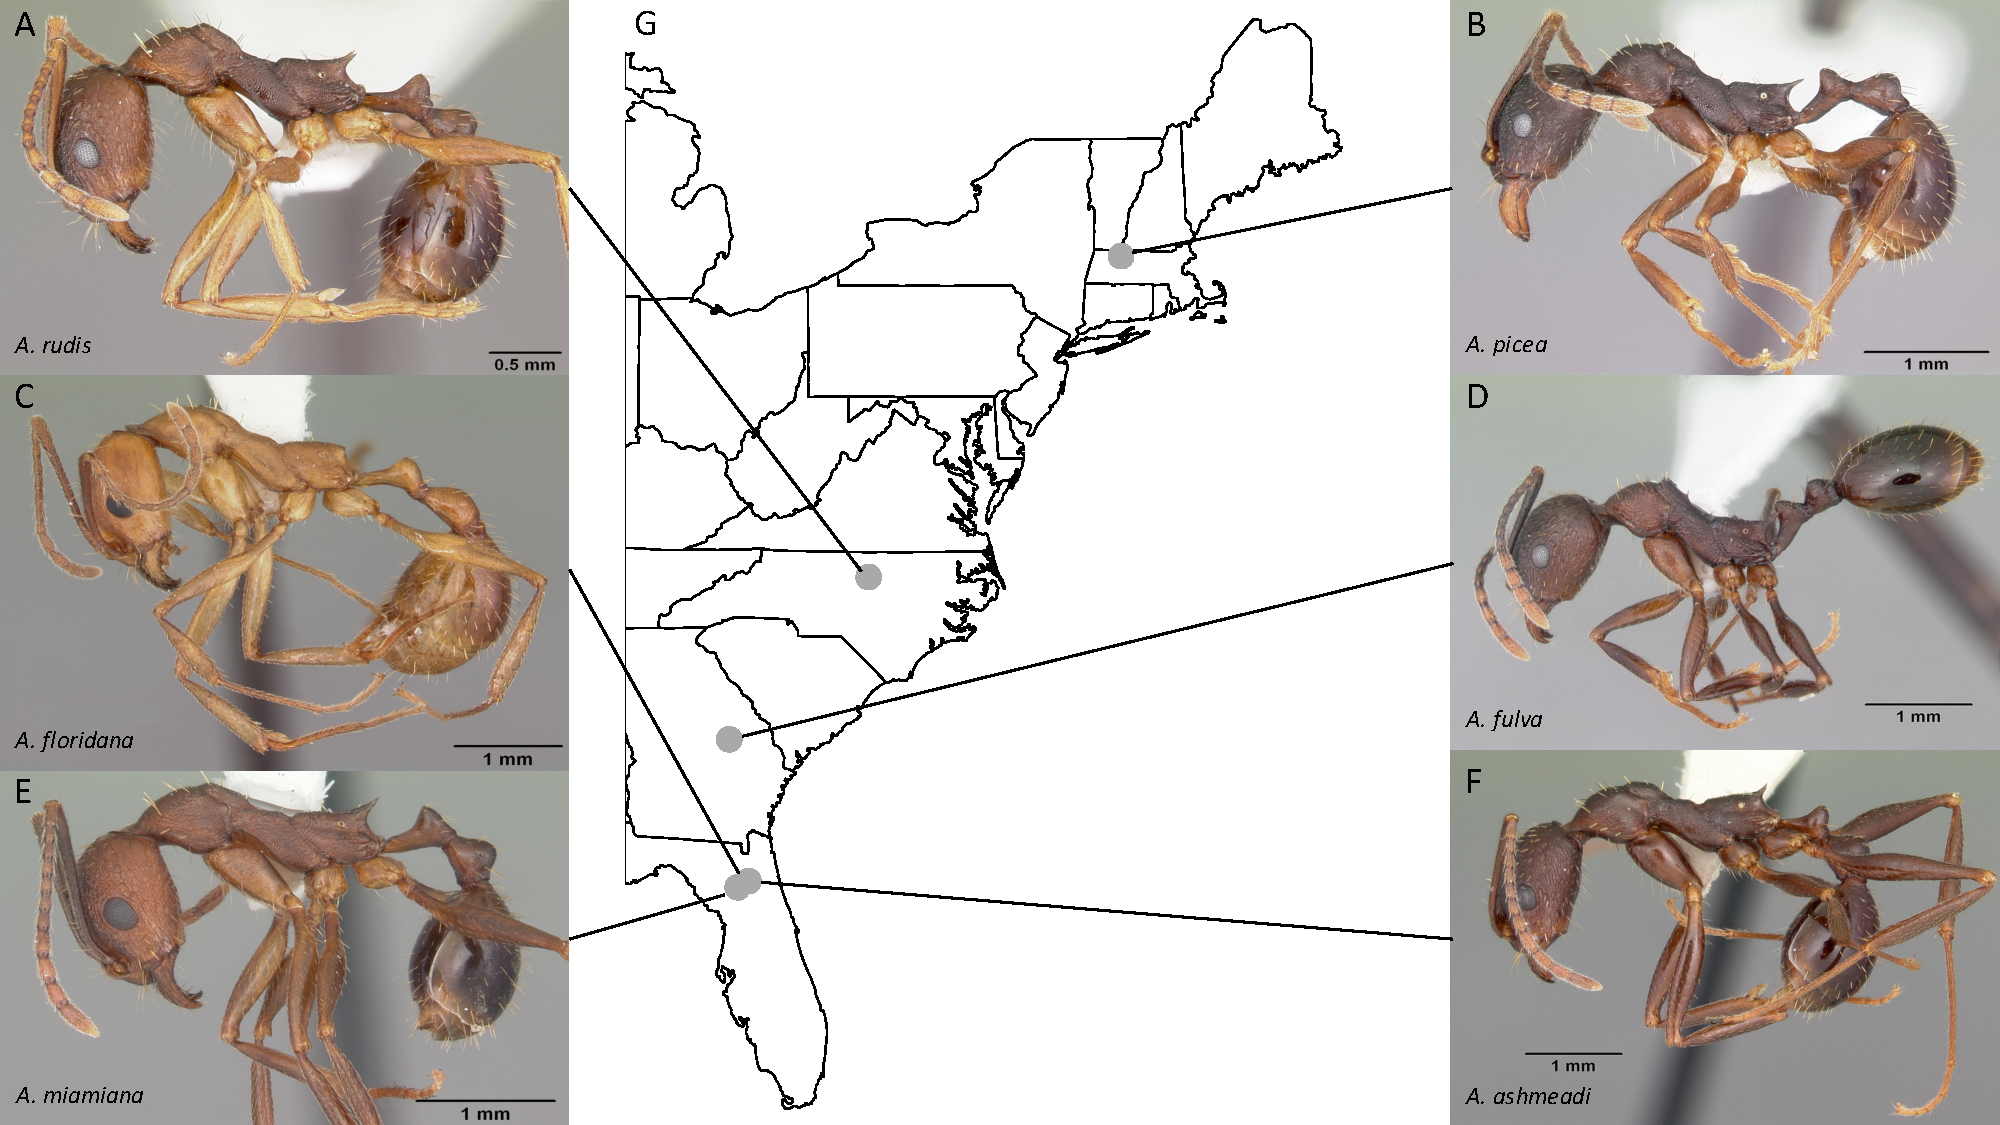
\includegraphics[width = 0.9\textwidth]{map_apg.pdf}
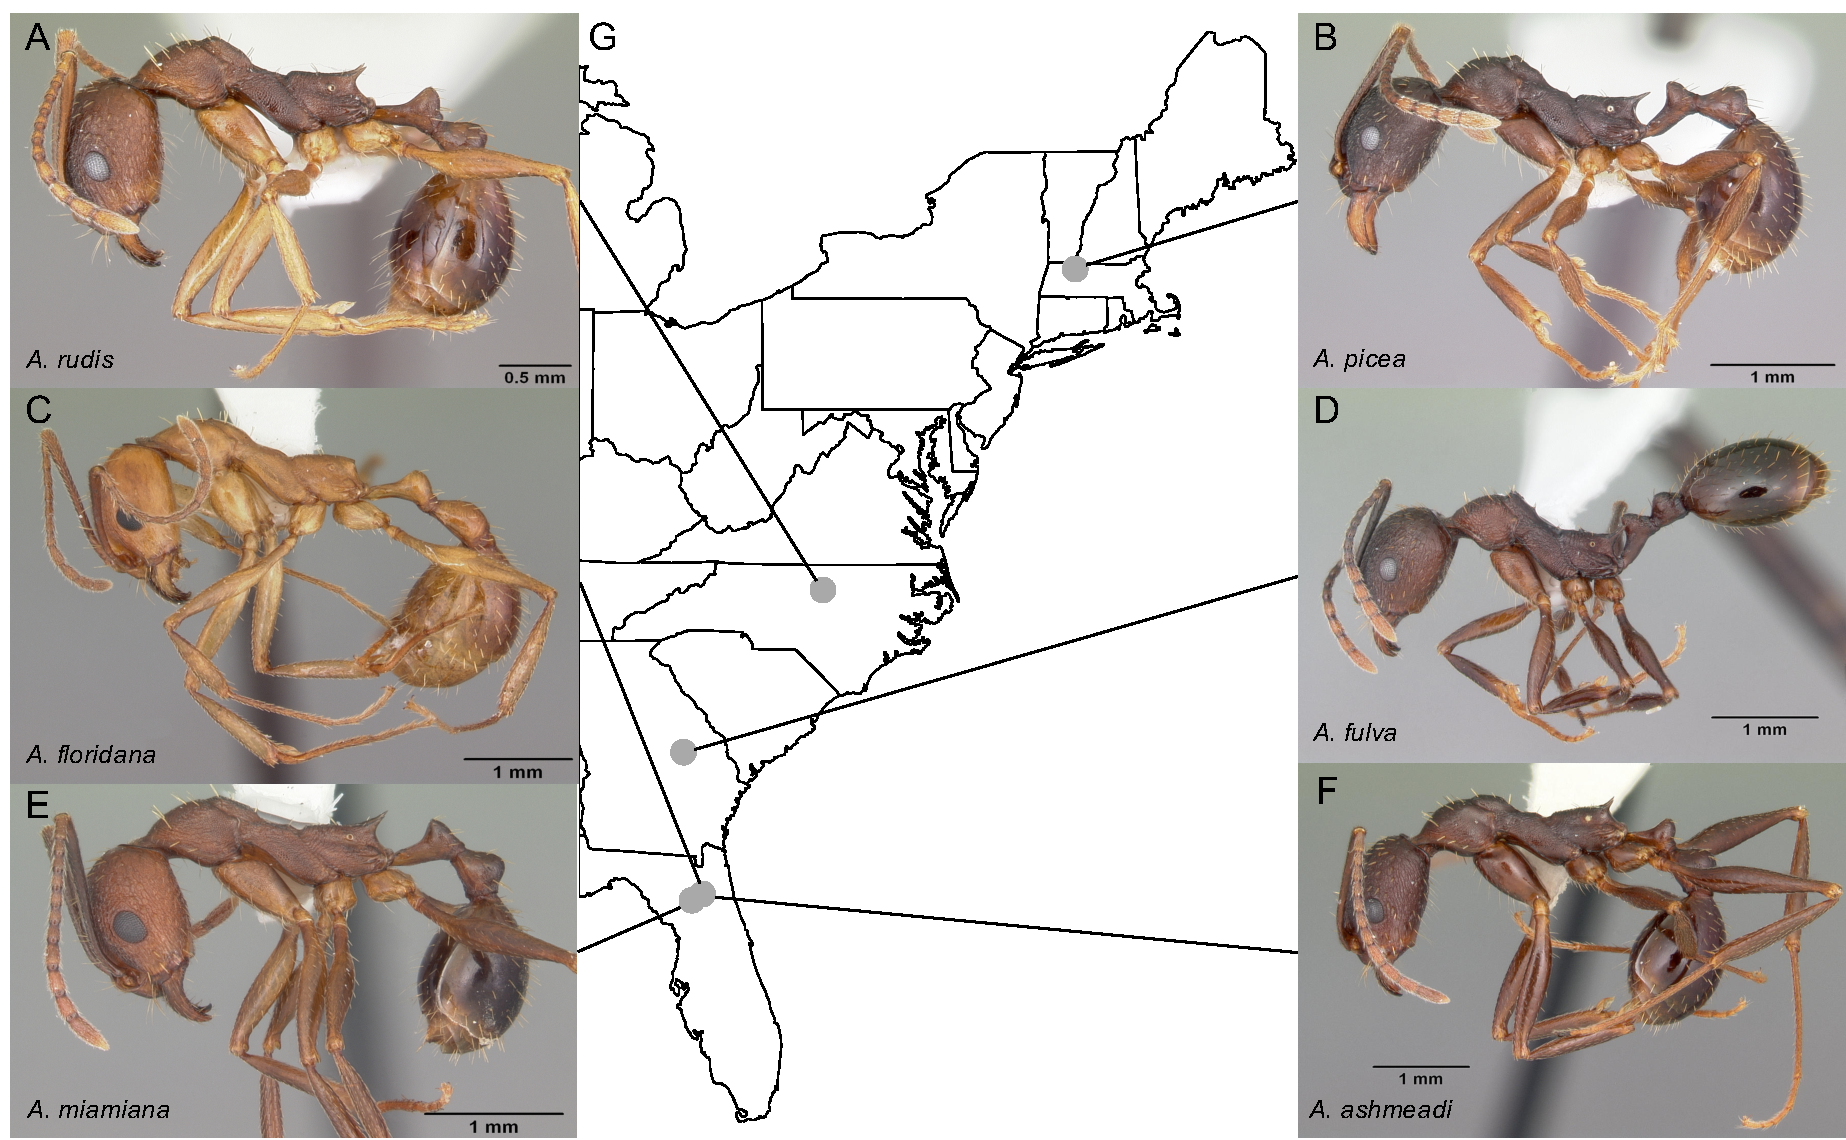
\includegraphics[width = 0.9\textwidth]{fig2.pdf}
\caption{We sampled seven colonies representing six species of
  \textit{Aphaenogaster}, including A) \textit{A. rudis}, B)
  \textit{A. picea}, C) \textit{A. floridana}, D) \textit{A. fulva},
  E) \textit{A. miamana} and F) \textit{A. ashmeadi} from G) sampling
  locations across eastern North America (see
  Table~\ref{tab:climate}). All photos by April Noble (available from
  http://www.antweb.org).}
\label{fig:sampling}
\end{figure}

Whole colony DNA was used to have sufficient concentrations for
sequencing. DNA was then extracted from each colony using methods
developed previously for genomic sequencing of whole colonies of
colonial mosquitos (\textit{Anopheles} spp.)  \citep{Neafsey2010} and
sequenced using an Illumina HiSeq 2500 at the Broad Institute
(Cambridge, MA, USA). A combination of fragment and jump sequences
were used to generate higher quality, long sequence reads. 

Raw sequences were processed to remove chimeric and contaminant
sequences, screened for contaminants by BLAST searches (using
\textit{blastn}) to identify sequences with likely matches to
non-target species (primarily \textit{Wolbachia} and
\textit{Mycoplasma}), and assembled using ALLPATHS-LG (version r48559)
\citep{Gnerre2011}. Additional assembly processing using PILON
(version 1.13) \citep{Walker2014} was applied to reduce base-call
errors and gaps in coverage. On average, across all seven genomes,
PILON reduced coverage gaps by 3.1\% or 3.9 Mb. GAEMR
(http://www.broadinstitute.org/software/gaemr/) software produced
summary statistics of the final assembled genomes. Once assembled,
repeat regions in the \emph{Aphaenogaster} genomes were deteced and
masked using \textit{Repeatmasker} (version 4.0.5 Institute for
Systems Biology).

%% % latex table generated in R 3.4.2 by xtable 1.8-2 package
% Tue Mar 20 17:26:28 2018
\begin{table}[ht]
\centering
\begin{tabular}{rrrrrr}
  \hline
 & Lat & Lon & Tmin (C) & Tmax (C) & Precip (mm) \\ 
  \hline
{\emph{Aphaenogaster ashmeadi}} & 29.79 & -82.03 & 6.11 & 33.13 & 1290.40 \\ 
  {\emph{Aphaenogaster floridana}} & 29.79 & -82.03 & 6.11 & 33.13 & 1290.40 \\ 
  {\emph{Aphaenogaster fulva}} & 32.69 & -82.51 & 1.83 & 33.81 & 1156.81 \\ 
  {\emph{Aphaenogaster miamiana}} & 29.66 & -82.30 & 5.87 & 32.75 & 1254.72 \\ 
  {\emph{Aphaenogaster picea}} & 42.60 & -72.58 & -11.11 & 28.12 & 1199.06 \\ 
  {\emph{Aphaenogaster rudis1}} & 36.02 & -78.98 & -1.82 & 31.60 & 1168.41 \\ 
  {\emph{Aphaenogaster rudis2}} & 36.02 & -78.98 & -1.82 & 31.60 & 1168.41 \\ 
   \hline
\end{tabular}
\caption{Climate variables for colony sample sites. Climate are 30 year normal values (1976-2016) for January minimum temperature (Tmin), July maximum temperature (Tmax) and total precipitation (Precip).} 
\label{tab:climate}
\end{table}

\input{table1.tex}

\subsection*{Analysis of Genomes along Climate Gradients}

After masking repeat regions, we applied MASH distance
\citep{Ondov2016} to measure pairwise dissimilarity of genomic
sequences. The MASH method extends a data compression and
dimensionality-reduction algorithm to generate estimates of sequence
similarity with low computational overhead. Briefly, the pairs of
genomic sequences were pre-processed into sets of k-mers of size 21
with the size of the non-redundant hashes retained set to 1,000. These
settings have been demonstrated to provide good representation of
genomic similarity with minimal computational costs
\citep{Ondov2016}. These sets were then used to estimate the Jaccard
similarity coefficient (the ratio of shared k-mers to total k-mers) of
subsampled k-mer pairs of genomes. This unbiased estimate of the
Jaccard similarity ($J$) was then used to calculate the dissimilarity
of the two genomes ($D$) as $D = 1 - J$. All Jaccard similarity
estimates had \textit{p}-values less than $10^{-14}$, which is below
the recommended $10^{-3}$ probability of observing values of $J$ due
to chance.


We used multivariate correlation analyses to examine biogeographic
patterns of ant genomes. Mantel tests of multivariate correlation of
distance matrices were used to examine correlations among ant genomes
and climate variables. Specifically, we used directional (H$_{\circ}$:
Mantel r $\leq$ 0) partial mantel tests, which calculate the
correlation between two distance matrices while controlling for the
covariance with other matrices \citep{Goslee2007}. First, we examined
the correlations between genomic similarity (MASH distance),
whole-genome size similarity (Euclidean distance of assembly size in
total base pairs) and climate variables (also using Euclidean
distance). Via partial Mantel tests, we were able to isolate the
correlation between genome size and climate by controlling for spatial
autocorrelation and potential phylogenetic patterns by including
geodesic and MASH distances as terms. 

We obtained previously sequenced ant whole genome and climate data
from a publicly available databases. Whole genome sequences for ants
were obtained from the NCBI Genome database (accessed August 2018, see
Supplementary Materials Table 1). Climatic
variables for each sampling location was obtained from the WorldClim
database (version 2.0) at a 2.5 arc minute spatial resolution from the
years 1970 to 2000 \citep{Fick2017}. Although used in the previous
analyses of ant genomes, two species, (\textit{W. auropunctata} and
\textit{M. pharaonis}), which did not have published location
information, were excluded from biogeographic analyses.

Using a permutational multivariate analysis of variance (PerMANOVA)
procedure, we parsed the individual variables that were correlated
with both genome size and MASH similarity. PerMANOVA is a flexible
multivariate analog of ANOVA that permits the use of a wider set of
similarity metrics to be used for the response matrix
\citep{Anderson2001}, such as the MASH distance. We ran a total of
10,000 permutations of the original distance matrices for each
statistical permutation procedure. We chose a subset of all possible
climate variables available via WorldClim for this analysis. A visual
inspection of the sampled climate variable correlations indicated that
the primary climate variables, mean annual temperature (MAT), minimum
temperature of the coldest month (Tmin), maximum temperature of the
hottest month (Tmax), annual precipitation (PA) and precipitation
seasonality (PS), represented the majority of climate variation
(Fig~\ref{fig:clim_cor}). Based on this, we only included these
variables, along with latitude and longitude coordinates, as factors
in the PerMANOVAs.

It is important to note that we are using assembly size as an
indicator of genome size. As genome size estimates are generally used
to set assembly size targets for whole genome sequencing efforts
\citep{Hare2011}, we expect there to be a high degree of correlation
between assembly size and genome size. Also, as a test of the
potential relationship between assembly size and true genome size, we
examined the correlation between the average assembly sizes of ant
genera that overlapped with flow cytometry estimates of those
published in \citet{Tsutsui2008a}. We found a marginally significant
correlation assembly size and flow cytometry at the genus level
(Spearman's $\rho$ = 0.57, \textit{p-value} = 0.076), which supports
the use of assembly size as a useful indicator of genome size.


\begin{figure}[ht]
%% 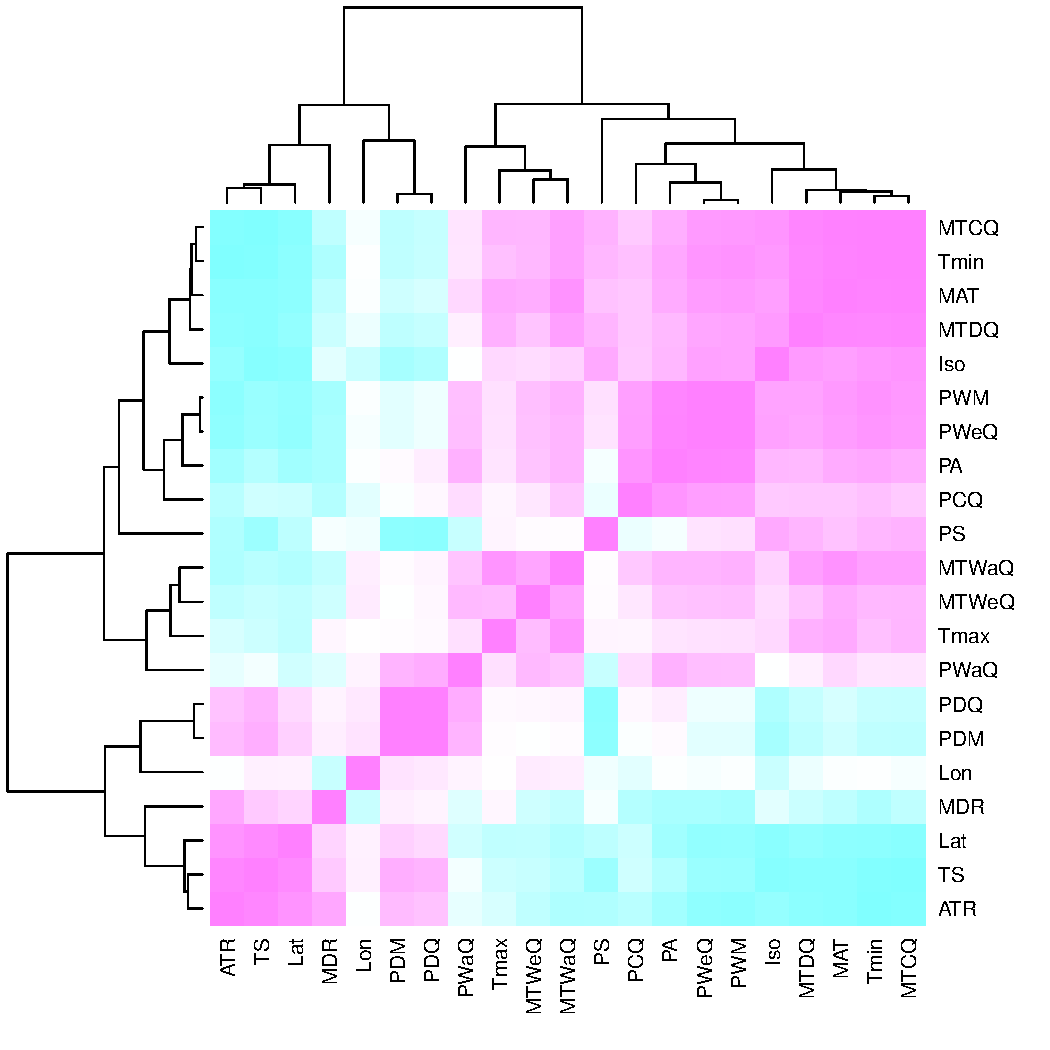
\includegraphics[width = 1\textwidth]{clim_cor.pdf}
\includegraphics[width = 1\textwidth]{fig3.pdf}
\caption{Heatmap of Pearson correlations among climate
  variables. Cells in the heatmap are colored by the correlation
  between the two variables that intersect at that location ranging
  from blue = -1 to white = 0 to pink = 1. The variables are arrayed
  by hierarchical clustering of the correlations, as shown by the
  dendrograms on the top and left side. For variable descriptions see
  Table~\ref{tab:wc_var}.}
\label{fig:clim_cor}
\end{figure}


\subsection*{Data, Computation and Statistics}

The raw and assembled genome sequences are currently archived at
Harvard Forest (Petersham, MA, USA) and in NCBI's genome database
(Genome Accessions NJRK00000000-NJRQ00000000 and BioSample Accessions
SAMN06892346-SAMN06892352). Genomic distance (MASH) computations were
run on the Odyssey cluster supported by the FAS Division of Science,
Research Computing Group at Harvard University. All analyses were
conducted in \textbf{R} \citep{RCoreTeam2017}. Analytical scripts for
the project have been versioned and archived (DOI:
10.5281/zenodo.1341982) and are available online at
https://zenodo.org/record/1341982. We used the \textit{vegan}
\citep{Oksanen2016} and \textit{ecodist} \citep{Goslee2007} packages
in R for multivariate analyses.

\section*{Results}

\subsection*{Genome Quality and Composition}

DNA extractions yielded substantial amounts of high quality DNA with
concentrations and quality scores ranging from 3.45\textendash5.39
ng$\mu$L$^{-1}$ and 4.05\textendash4.27 ng$\mu$L$^{-1}$,
respectively. All genome assemblies displayed good coverage, with an
average of 70\% across all genomes (Table
\ref{tab:assemblystats}). Across all species, the length of the
shortest contig at 50\% of the genome (i.e. N50) was 18,864 bases;
average assembly GC content was 38.18\%; and average genome size was
370.45 Mb.  Using GAEMR's BLAST feature to conduct a search of the
contigs against the NCBI's nucleotide sequence database, we discovered
that 38.98\% and 22.04\% of the top hits were ``ant'' and
\textit{Aphaenogaster}, respectively. The \textit{Aphaenogaster}
genomes compared well with other ant genome sequences. The sizes of
the \textit{Aphaenogaster} genomes were within the range of other ant
genomes based on size from both flow cytometry \citep{Tsutsui2008a}
and the previously sequenced ant genomes available in NCBI
(Fig~\ref{fig:ncbi_compare}).


%%% assembly statistics table. 
%% \input{assembly_stats}
\input{table2.tex}

\begin{figure}[ht]
%% \includegraphics[width = 0.90 \textwidth]{ncbi_gaga_compare.pdf} 
\includegraphics[width = 0.90 \textwidth]{fig4.pdf}
\caption{The size of sequenced \textit{Aphaenogaster} genomes were
  within the size range of previously published observed or estimated
  genomes of ants. Frequency distribution of previously published
  genome size estimates using flow cytometry from \cite{Tsutsui2008a}
  and those available via NCBI (accessed August 2018). Vertical lines
  identify the sizes of the \textit{Aphaenogaster} assemblies (see
  Table~\ref{tab:assemblystats}).}
\label{fig:ncbi_compare}
\end{figure}


Using the MASH genomic distances, we observed patterns of genomic
similarity that were in line with expectations of ant
relatedness. Sequences formed groups that corresponded with
subfamilies (Fig~\ref{fig:all_heat}). \textit{Aphaenogaster} clustered
with other genera from the Myrmicinae and, in general, subfamily level
clustering tended to follow previously observed patterns of subfamily
relatedness \citep{Bolton2006, Moreau2006, Ward2014}.  The
\emph{Aphaenogaster} sequences formed a single cluster containing only
\emph{Aphaenogaster} species and displayed intra-generic levels of
genomic variance comparable to other genera s(e.g.,
\textit{Trachymyrmex} spp.). The separation of the two
\textit{A. rudis} species was initially surprising, as these two
samples were collected at the same site (Duke Forest, NC USA) and were
identified as the same species based on their morphological
characteristics \citep{Ellison2012, Demarco2016}. However, two recent
studies of targeted gene regions have demonstrated the polyphyletic
nature of \textit{Aphaenogaster rudis}.  One study of the evolution of
the subfamily Myrmicinae observed that the genus as a whole could be
split into at least four different lineages \citep{Ward2015}. Another,
more detailed study of the genus in North America found that multiple
individuals of \textit{A. rudis} separated out into distinct
groupings, each with other species, specifically, individuals of
\textit{A. rudis} from North Carolina (USA) were observed to form
distinct clusters with individuals of \textit{A. carolinensis},
\textit{A. miamiana}, \textit{A. lamellidens} and \textit{A. texana}
\citep{Demarco2016}.


\begin{figure}[ht]
%% 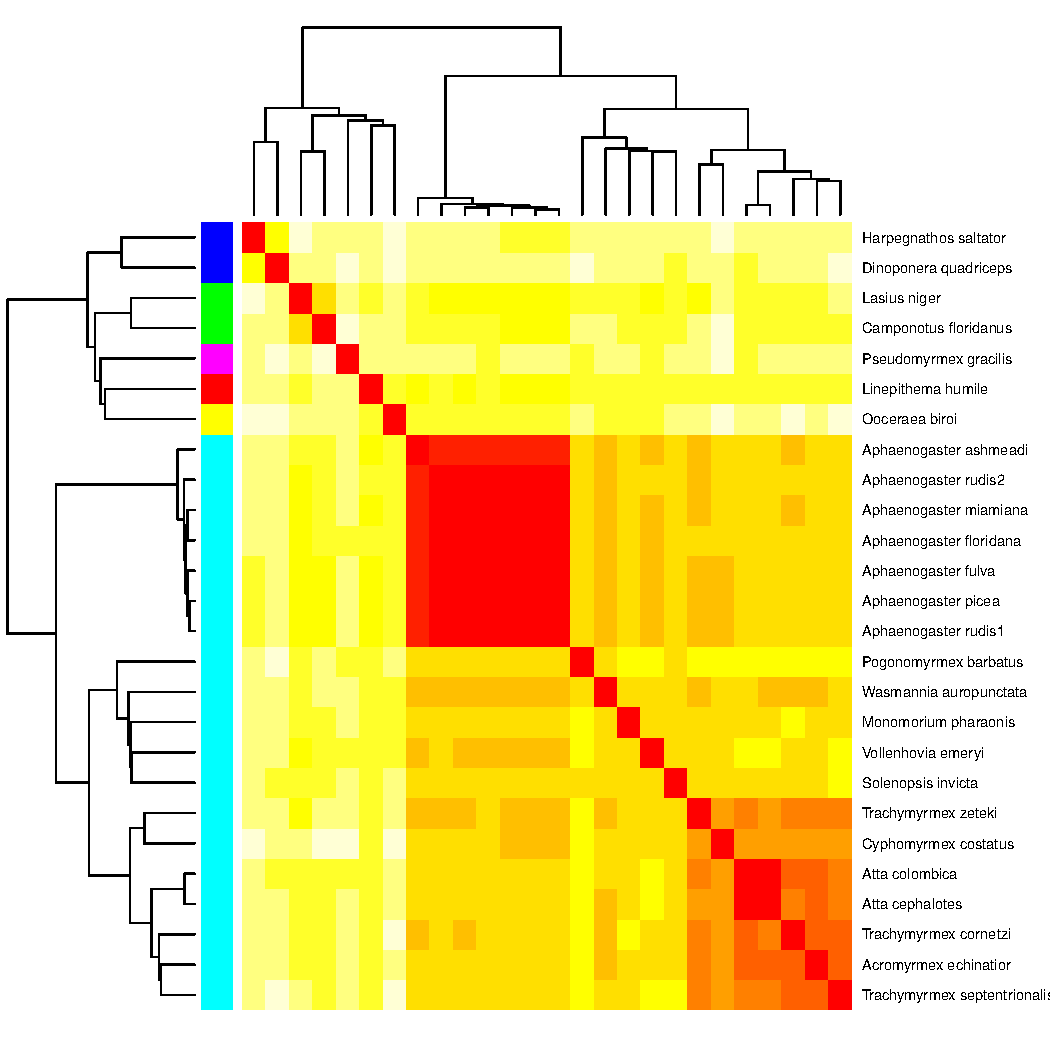
\includegraphics[width = 1\textwidth]{ncbi_heat.pdf}
\includegraphics[width = 1\textwidth]{fig5.pdf}
\caption{Heatmap of the MASH genomic distances of the
  \textit{Aphaenogaster} species that we sampled together with other
  ant species in NCBIs. Heat colors shown in the central matrix range
  from high (white = 1) through moderate (orange = 0.5) to low (red =
  0) genomic distance; the diagonal is entirely red because it
  illustrates the distance of each sequence to itself. The cladograms
  on the left and top show hierarchical clustering of the
  genomes. Colors shown to the left of the matrix indicate ant
  subfamilies:  \emph{Ponerinae} (dark blue), \emph{Formicinae}
  (green), \emph{Pseudomyrmecinae} (pink), \emph{Dolichoderinae}
  (red), \emph{Dorylinae} (yellow), \emph{Myrmicinae} (light blue).}
\label{fig:all_heat}
\end{figure}


\subsection*{Biogeographic Patterns of Ant Genomes}


%% \input{wc_vars}
\input{table3.tex}

After controlling for both spatial autocorrelation and potential
phylogenetic patterns, we found a marginally significant, positive
correlation between ant genome size similarity and climate similarity
(Mantel R = 0.14, \textit{p-value} = 0.055). Although genome size
similarity and MASH genome similarity were not significantly
correlated (Mantel R = 0.08, \textit{p-value} = 0.217), we included
MASH as a covariate in addition to geodesic distance because previous
research indicated that genome size is associated with phylogenetic
relatedness \citep{Alfsnes2017}. We found that different spatial and
climatic variables were associated with the size similarity of ant
genomes. Longitude but not latitude was a significant predictor of
genome size (Table~\ref{tab:perm_f_size}). Temperature of the coldest
(Tmin) and hottest (Tmax) month and total annual precipitation (PA),
were significant predictors, but neither mean annual temperature (MAT)
nor precipitation seasonality (PS) were significant predictors of
genome size. Overall, Tmin had the highest correlation with an
\textit{R}$^2$ of 0.23. Examining the correlation between genome size
and Tmin, we observed a negative correlation with genome size tending
to increase as minimum temperature decreased
(Fig~\ref{fig:size_tmin}). When the newly sequenced
\textit{Aphaenogaster} genomes were excluded from the analysis, only
annual precipitation (PA) was a significant predictor of genome size
similarity (see Supplementary Materials
Table 2).

%% \input{perm_f_size}
\input{table4.tex}

\begin{figure}[ht]
%% 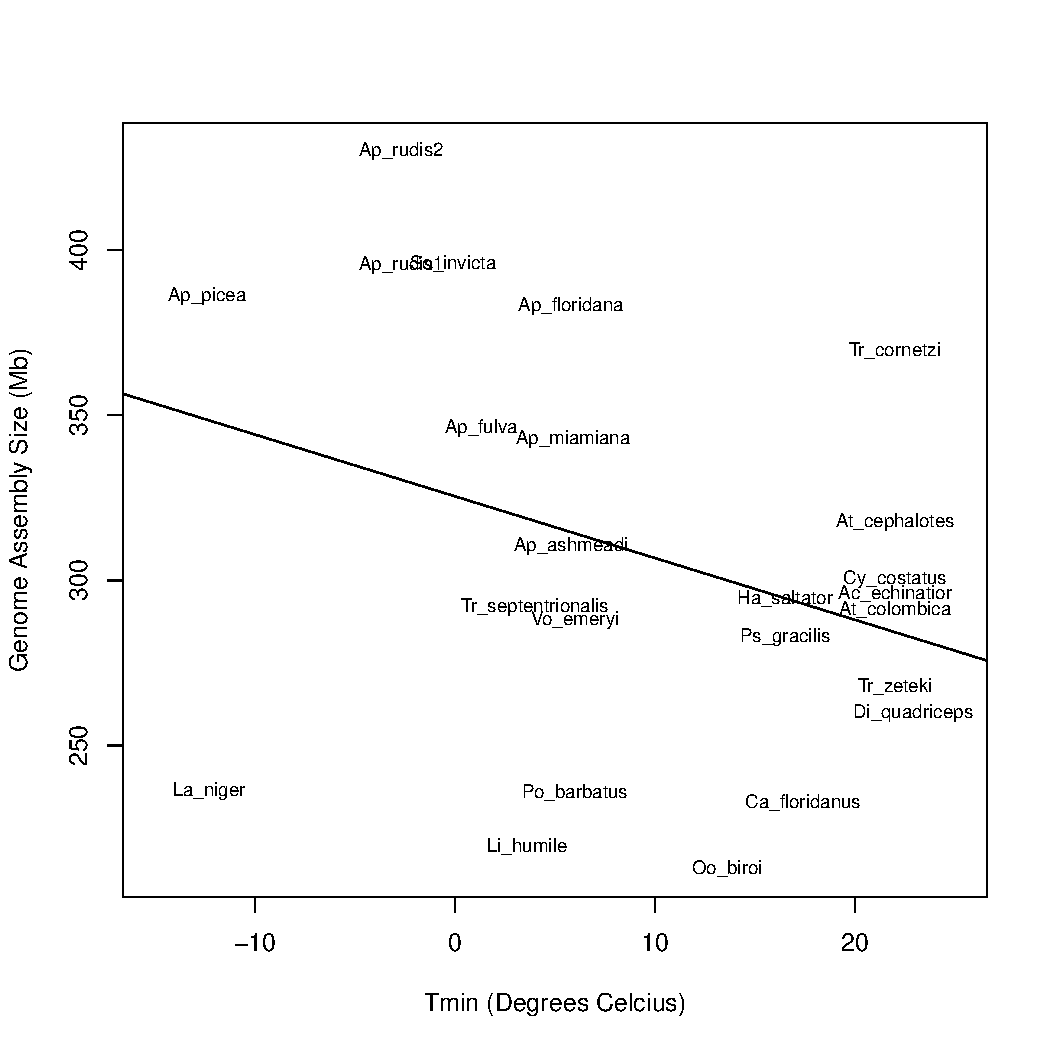
\includegraphics[width = 1\textwidth]{size_tmin.pdf}
\includegraphics[width = 1\textwidth]{fig6.pdf}
\caption{Bivariate plot showing the correlation between ant assembly
  size and minimum temperature of the coldest month (Tmin). Ants from
  locations with lower minimum temperatures tended to have larger
  genomes.}
\label{fig:size_tmin}
\end{figure}


\newpage
\clearpage

\section*{Discussion}

We have produced seven draft whole-genome sequences of six species of
ants in the genus \textit{Aphaenogaster}. The addition of the
\textit{Aphaenogaster} sequences increases the breadth of global ant
genomic sampling, as these are the first whole-genomes from a
previously un-sequenced genus, adding to the sequences of the diverse
``formicoid'' clade, which contains 90\% of all extant ant species
\citep{Ward2014}.  Our genomic sequences were comparable in quality to
other ant and insect genomes and the patterns of genomic similarity
were in line with expectations based on current ant systematics. With
the addition of the new \textit{Aphaenogaster} sequences, our initial
biogeographic analysis revealed that ant genomes from more similar
climates have more similarly sized genomes with minimum temperatures
having the strongest correlation with genome size, which is consistent
with the hypothesis that climate has been a force shaping ant genome
size.

Although correlative, our genome analysis results are consistent with
the hypothesis that ants from regions with more similar climates tend
to have similar sized genomes. Previous studies have observed
physiological and ecological responses of ants to climate gradients
and shifting temperatures \citep{Warren2013, Stanton-Geddes,
  Diamond2016, Nguyen2017, HelmsCahan2017, Diamond2017, Penick2017}
that could act as agents of selection or as environmental filters. For
example, \cite{Warren2013} found that cold, but not warm, temperatures
limited shifts in the distributions of \textit{A. picea} and
\textit{A. rudis}. \cite{Diamond2016} reported that the rate of
colonization and occupancy of nests by \textit{Aphaenogaster} species
in a five-year experimental warming study \citep{Pelini2014} declined
with temperature in the warm, southern study site (Duke Forest, NC,
USA) but not in the cooler, northern study site (Harvard Forest, MA,
USA). In addition to the direct impacts of climate, some studies
support the importance for the indirect effects of climate via biotic
interactions. For example, the distribution of the species
\textit{Atta texana} is limited by the cold-tolerance of its fungal
symbiont, cultivars of the genus \textit{Attamyces}
\citep{Mueller2011}. The evolution of the ant-fungus relationship has
led to reductions in some ant species ranges by cold temperatures.

Specific to temperature, we found support for increasing genome size
with colder temperatures. We are cautious to offer possible mechanisms
for this trend. In the general context of arthropods, genome size
appears to be influenced by a complex array of selection pressures, as
evidenced by the recent study by \citet{Alfsnes2017}, which found that
genome size patterns varied greatly among major arthropod taxa with
high potential for different mechanisms affecting genome size. For
example, insects displayed clear phylogenetic correlations with genome
size while genome size patterns in crustaceans were nearly independent
of phylogeny but strongly related to biogeographic gradients
(e.g. decreasing genome size with increasing maximum observed
latitude). In addition, \citet{Hultgren2018} found evidence for
increasing genome size with latitude in crustaceans but not decapods,
adding another example of the potential complexity of genome size as
an adaptive trait.

There is the potential for both direct and indirect selection for
increased genome size in colder conditions. \citet{Hessen2010} has
proposed that there is a complex set of relationships among genome
size, developmental rate, cell size and body size and that selection
can act at different points in this causal network. One possible
direct pathway is that increased expression of gene products that deal
with cold stress could lead to larger genomes via whole genome or
individual gene duplications \citet{Dufresne2011}. Previous work with
\textit{Aphaenogaster} supports this hypothesis, as
\citet{Stanton-Geddes} found that exposure to extreme cold induced
expression of genes in the cold-climate \textit{A. picea} more so than
in \textit{A. carolinensis} (a more southern, warm climate species).
An example of a possible indirect pathway is that cold could select
for increased body size to deal with heat-loss in cold conditions
\citep{Brown2004}, which could lead to larger genome sizes. There is
evidence of cold selecting for greater body size (i.e. Bergmann's
Rule) in ants \citep{Heinze2003, Bernadou2016}, and some have
hypothesized that increased body size could lead indirectly to
increased genome size via increased cell size \citep{RyanGregory2005};
however, the most recent, broad analysis of genome size in ants (that
we are aware of) did not find support for a relationship between ant
genome size and body size after controlling for phylogenetic patterns
\citep{Tsutsui2008a}. Therefore, assuming that our analysis adequately
controlled for phylogenetics, indirect selection on genome size via
body size is not a likely explanation for our observed relationship
between genome size and temperature.

It is important to keep in mind that the climate related genomic
patterns observed in this study should be considered an initial view
of possible biogeographic patterns in ant genomes. As the addition of
the these sequences had a marked impact on the statistical results of
the climate analysis (see Supplementary Materials
Table 2), we expect that further sequencing
work will continue to enhance our understanding of the ecological
genomics of ants. Also, these findings should be tested with
additional sequencing efforts, as we could not control for several
potentially important intercorrelated variables. Factors such as
sampling bias and sequencing methodology (e.g. 454 versus Illumina)
also varied among sequencing efforts, which could have contributed to
some of the observed correlations with climate. We did not attempt to
control for these factors statistically due to the limitations of the
current ant genome sample size. Future work should methodologically
and/or statistically control for such sources of variation in ant
genomes as more sequences become available to illucidate clearer
patterns and resolve underlying ecological and evolutionary
mechanisms.


\section*{Conclusion}

Although we have increased the total number of sequenced ant genomes
by over 30\%, the total number of ant sequences analyzed here is still
a relatively small sample (n = 26) of the estimated $>$16,000 ant
species and subspecies (www.antweb.org, accessed 20 Aug 2018). Efforts
such as The Global Ant Genomics Alliance (GAGA)\citep{Boomsma2017},
which aims to greatly increase the number of ant species sequenced
from across the world, will provide additional resources for
ecological genomics studies. Further work investigating the variation
in genomic content and mapping of target coding regions from previous
physiological \citep{Nguyen2017}, biochemical \citep{HelmsCahan2017},
and transcriptomic \citep{Stanton-Geddes} studies of
\textit{Aphaenogaster} and other ant species will inform predictions
of how these species, and the ecosystems that they inhabit, may
respond to ongoing climatic change. For instance, determining the
genomic factors underlying the temperature response of ant assemblages
to climatic gradients \citep{Warren2013, Diamond2016, Diamond2017}
could provide useful insights into the response of these important
organisms to non-analog ecosystem states and idiosyncratic community
responses \citep{Bewick2014a}. In addition, as species distribution
models have been significantly improved by the inclusion of genetic
information \citep{Ikeda2016}, an ecological genetics approach that
couples ant genomic and ecologically relevant data will provide a
useful window into the response of many terrestrial ecosystems to a
changing climate.


\section*{Acknowledgments}

Thank you to the genome sequencing team at the Broad Institute
(particularly, James Bochicchio, Sarah Young, Terrance Shay and
Caroline Cusick) and to Manisha Patel at Harvard Forest's Torrey Lab
for assistance in obtaining and properly storing ant colonies.

%% This work was supported by a US National Science Foundation
%% Dimensions of Biodiversity grant (DEB 11-36646) to NJS, RRD, AME,
%% NJG and SHC.

%% Our manuscript was written with \LaTeX~in \emph{Emacs} and
%% \emph{Overleaf} (\url{www.overleaf.com}).
%% We used the Mendeley citation manager.
%% So long and thanks for all the fish.


\newpage
\clearpage

\bibliography{apGenomes}

%% \clearpage

%% \section*{Supplementary Materials}

%% \setcounter{figure}{0}
%% \setcounter{table}{0}

% Table 1
%% % latex table generated in R 3.4.4 by xtable 1.8-2 package
% Tue Jul 10 16:48:17 2018
\begin{table}[ht]
\centering
\begin{tabular}{rllll}
  \hline
 & BioProject Accession & BioSample Accession & Lat & Lon \\ 
  \hline
{\emph{Acromyrmex echinatior}} & PRJNA62733 & SAMN02953789 & -79.696513 & 9.1164638 \\ 
  {\emph{Atta cephalotes}} & PRJNA48091 & SAMN02953774 & -79.696513 & 9.1164638 \\ 
  {\emph{Atta colombica}} & PRJNA343260 & SAMN03982875 & -79.696513 & 9.1164638 \\ 
  {\emph{Camponotus floridanus}} & PRJNA50201 & SAMN02953777 & -81.5431872 & 24.6245746 \\ 
  {\emph{Cyphomyrmex costatus}} & PRJNA343963 & SAMN03982885 & -79.696513 & 9.1164638 \\ 
  {\emph{Dinoponera quadriceps}} & PRJNA301625 & SAMN02869781 & -79.8697222 & 9.4008333 \\ 
  {\emph{Harpegnathos saltator}} & PRJNA50203 & SAMN00016742 & 75.7138884 & 15.3172775 \\ 
  {\emph{Lasius niger}} & PRJNA269328 & SAMN03253098 & 37.6172999 & 55.755826 \\ 
  {\emph{Linepithema humile}} & PRJNA45799 & SAMN02767796 & -122.0230146 & 37.2638324 \\ 
  {\emph{Monomorium pharaonis}} & PRJDB3164 & SAMD00020277 & NA & NA \\ 
  {\emph{Ooceraea biroi}} & PRJNA275884 & SAMN02428046 & 127.6809317 & 26.2124013 \\ 
  {\emph{Pogonomyrmex barbatus}} & PRJNA45797 & SAMN02953770 & -100.3898876 & 20.5888184 \\ 
  {\emph{Pseudomyrmex gracilis}} & PRJNA377720 & SAMN03219222 & -70.8119953 & -11.7668705 \\ 
  {\emph{Solenopsis invicta}} & PRJNA49629 & SAMN02953778 & -83.357567 & 33.9519347 \\ 
  {\emph{Trachymyrmex cornetzi}} & PRJNA343972 & SAMN03982882 & -79.696513 & 9.1164638 \\ 
  {\emph{Trachymyrmex septentrionalis}} & PRJNA343973 & SAMN03982881 & -84.2807329 & 30.4382559 \\ 
  {\emph{Trachymyrmex zeteki}} & PRJNA343251 & SAMN03982884 & -79.696513 & 9.1164638 \\ 
  {\emph{Vollenhovia emeryi}} & PRJDB3517 & SAMD00026325 & -100.3898876 & 20.5888184 \\ 
  {\emph{Wasmannia auropunctata}} & PRJDB3443 & SAMD00024919 & NA & NA \\ 
   \hline
\end{tabular}
\caption{NCBI genome database accession information for the previously sequenced ant genomes and coordinates for species those species that could be obtained from the published literature.} 
\label{tab:ncbi_info_locs}
\end{table}

%% \label{tab:ncbi_info_locs}
% Table 2
%% \input{perm_f_size_napg} 
%% \label{tab:perm_f_size_napg}

%%% % latex table generated in R 3.4.2 by xtable 1.8-2 package
% Fri Dec 15 14:16:56 2017
\begin{table}[ht]
\centering
\begin{tabular}{lll}
  \hline
Ant Species & BioProject Accession & BioSample Accession \\ 
  \hline
Acromyrmex echinatior & PRJNA62733 & SAMN02953789 \\ 
  Atta cephalotes & PRJNA48091 & SAMN02953774 \\ 
  Atta colombica & PRJNA343260 & SAMN03982875 \\ 
  Camponotus floridanus & PRJNA50201 & SAMN02953777 \\ 
  Cyphomyrmex costatus & PRJNA343963 & SAMN03982885 \\ 
  Dinoponera quadriceps & PRJNA301625 & SAMN02869781 \\ 
  Harpegnathos saltator & PRJNA50203 & SAMN00016742 \\ 
  Lasius niger & PRJNA269328 & SAMN03253098 \\ 
  Linepithema humile & PRJNA45799 & SAMN02767796 \\ 
  Monomorium pharaonis & PRJDB3164 & SAMD00020277 \\ 
  Ooceraea biroi & PRJNA275884 & SAMN02428046 \\ 
  Pogonomyrmex barbatus & PRJNA45797 & SAMN02953770 \\ 
  Pseudomyrmex gracilis & PRJNA377720 & SAMN03219222 \\ 
  Solenopsis invicta & PRJNA49629 & SAMN02953778 \\ 
  Trachymyrmex cornetzi & PRJNA343972 & SAMN03982882 \\ 
  Trachymyrmex septentrionalis & PRJNA343973 & SAMN03982881 \\ 
  Trachymyrmex zeteki & PRJNA343251 & SAMN03982884 \\ 
  Vollenhovia emeryi & PRJDB3517 & SAMD00026325 \\ 
  Wasmannia auropunctata & PRJDB3443 & SAMD00024919 \\ 
   \hline
\end{tabular}
\caption{NCBI genome database accession information for the previously sequenced ant genomes.} 
\end{table}

%%% % latex table generated in R 3.4.4 by xtable 1.8-2 package
% Tue Jul 10 12:09:18 2018
\begin{table}[ht]
\centering
\begin{tabular}{rrr}
  \hline
 & Lon & Lat \\ 
  \hline
{\emph{Acromyrmex echinatior}} & 9.12 & -79.70 \\ 
  {\emph{Atta cephalotes}} & 9.12 & -79.70 \\ 
  {\emph{Atta colombica}} & 9.12 & -79.70 \\ 
  {\emph{Camponotus floridanus}} & 24.62 & -81.54 \\ 
  {\emph{Cardiocondyla obscurior}} & -19.92 & -43.94 \\ 
  {\emph{Cyphomyrmex costatus}} & 9.12 & -79.70 \\ 
  {\emph{Dinoponera quadriceps}} & 9.40 & -79.87 \\ 
  {\emph{Formica selysi}} & 46.58 & 10.32 \\ 
  {\emph{Harpegnathos saltator}} & 15.32 & 75.71 \\ 
  {\emph{Lasius niger}} & 55.76 & 37.62 \\ 
  {\emph{Linepithema humile}} & 37.26 & -122.02 \\ 
  {\emph{Ooceraea biroi}} & 26.21 & 127.68 \\ 
  {\emph{Pogonomyrmex barbatus}} & 20.59 & -100.39 \\ 
  {\emph{Pseudomyrmex gracilis}} & -11.77 & -70.81 \\ 
  {\emph{Solenopsis invicta}} & 33.95 & -83.36 \\ 
  {\emph{Trachymyrmex cornetzi}} & 9.12 & -79.70 \\ 
  {\emph{Trachymyrmex septentrionalis}} & 30.44 & -84.28 \\ 
  {\emph{Trachymyrmex zeteki}} & 9.12 & -79.70 \\ 
  {\emph{Vollenhovia emeryi}} & 20.59 & -100.39 \\ 
   \hline
\end{tabular}
\caption{Coordinates obtained from the literature published for the ant genome sequences used in the biogeographic analyses.} 
\end{table}
 

\end{document}
